\clearpage
\section{Original detector-to-window gas path}
The source-native detector top and window underside have opposed surface normals and a 3.873750 mm separation. Their actual triangular meshes were intersected after conservatively excluding the projected bounding boxes of all source solids crossing the gap. Of the 0.995800 mm$^2$ detector gas face, 0.694600 mm$^2$ is represented by 301 common projected polygons; the source mesh and CAD face-area disagreement is 0.1711\% for the window and negligible for the detector. The old interstage gas columns terminate below the new paths, and no source face or modeled area is reused for the same gas mechanism.

With a 300 K window assumption, 100 Pa krypton and accommodation 0.8, this subset contributes 0.112833 mW into the die in one matched-power coupled calculation. The original 752 ceramic P1 columns are retained, prior overlapping gas proxies are disabled, and gray radiation remains a separate proxy. At 0.595668 W electrical input and 2 mW die load, the modeled die, stage-2 cold-interface and carrier nodes are 218.693303, 218.605250 and 218.623662 K respectively. The die is 0.034196 K warmer than the preceding partial-cavity result. Independent stage and whole-package energy residuals are below $1.1\times10^{-9}$ W.

\begin{figure}[htbp]
\centering
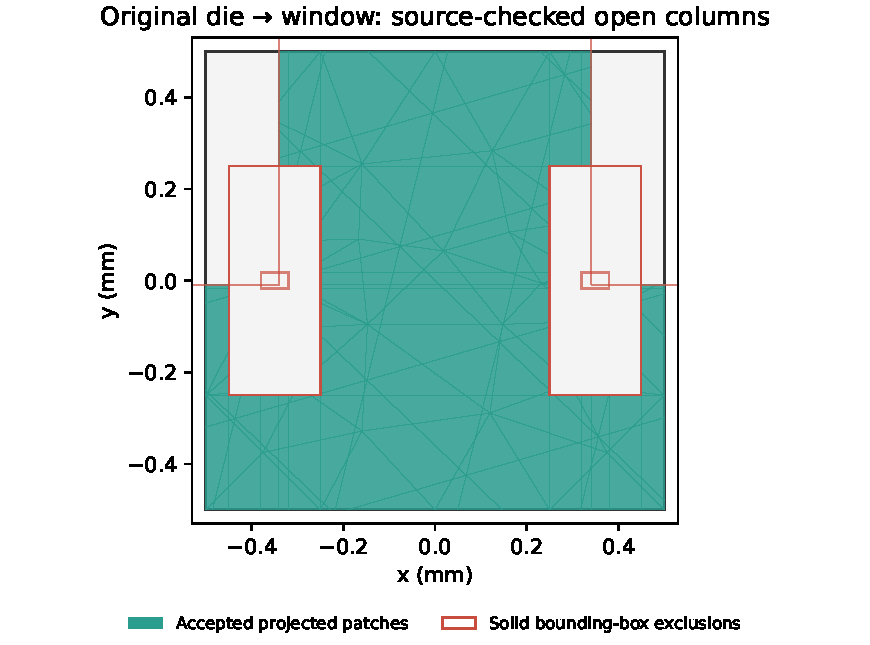
\includegraphics[width=.63\textwidth]{figures/v327_die_window_visibility.pdf}
\caption{Actual source-mesh die/window common projection. Green polygons are accepted straight geometric columns; red outlines conservatively exclude source contact and bond-wire bounding boxes. These columns are not molecular trajectories or a complete gas field.}
\end{figure}

The earlier independent-audit label \texttt{top\_K} refers to the carrier node, not the stage-2 cold-interface node; the distinction is made explicitly here. The modeled two-sided gas patches now cover 31.199236 mm$^2$, or 3.45424\% of registered gas-facing area. The remaining gas surfaces are adiabatic only in this conditional scenario. Lateral gas transport, actual window temperature and contact properties remain unqualified; these results are not complete-cavity or experimental device predictions. Historical gas-flux and three-dimensional metal-electrical gates remain failed.
